%%%%%%%%%%%%%%%%%%%%%%%%%%%%%%%%%%%%%%%%%%%%%%%%%%%%%%%%%%%%%%%%%%%%%%
% 
% 	Template for Producing ASP-DAC 2014 Proceedings
% 
%%%%%%%%%%%%%%%%%%%%%%%%%%%%%%%%%%%%%%%%%%%%%%%%%%%%%%%%%%%%%%%%%%%%%%
% History
% ??/??/?? Designed by Hiroaki Kunieda (ASP-DAC '97 Publication Chair)
% 09/22/97 Modified and small bug fixed by Masaharu Imai 
% 	   (ASP-DAC '98 Publication Chair)
% 11/02/98 Modified by Tsuyoshi Isshiki
% 	   (ASP-DAC 2000 TPS Secretary)
% 7/24/00 Modified by Kiyoharu Hamaguchi
% 	   (ASP-DAC 2001 Publication chair)
% 6/18/02 Modified by Kazutoshi Kobayashi
% 	   (ASP-DAC 2003 Publication Co-Chair)
% 5/27/03 Modified by Kiyoharu Hamaguchi
% 	   (ASP-DAC 2004 TPC secretary)
% 6/10/03 Modified by Kazutoshi Kobayashi for Latex2e
% 	   (ASP-DAC 2004 Publication Co-Chair)
% 6/01/05 Modified by Nozomu Togawa
% 	   (ASP-DAC 2006 Publication Chair)
% 6/01/06 Modified by Hiroyuki Ochi
% 	   (ASP-DAC 2007 Publication Chair)
% 5/30/08 Modified by Nozomu Togawa
% 	   (ASP-DAC 2009 Publication Co-Chair)
% 4/30/10 Modified by Masashi Imai
% 	   (ASP-DAC 2011 Publication Chair)
% 3/20/12 Modified by Masashi Imai
% 	   (ASP-DAC 2014 Publication Chair)
%%%%%%%%%%%%%%%%%%%%%%%%%%%%%%%%%%%%%%%%%%%%%%%%%%%%%%%%%%%%%%%%%%%%%%
% If you have any problem, please contact ASP-DAC 2014 Publication
% Co-Chairs by E-mail at ``aspdac2014-tpc@mls.aspdac.com.''
%%%%%%%%%%%%%%%%%%%%%%%%%%%%%%%%%%%%%%%%%%%%%%%%%%%%%%%%%%%%%%%%%%%%%%
%
\documentclass[twocolumn]{article}
%% If you use dvips and ps2pdf, please use Postscript font 
%% and uncomment the line below.
%%\usepackage{times}
\usepackage{url}
\usepackage{amsmath}
\usepackage{amsthm}
\usepackage{amsfonts}
\usepackage{subfig}
\usepackage{graphicx}
\pagestyle{empty}
\newtheorem{theorem}{Theorem}[section]
\newtheorem{lemma}[theorem]{Lemma}
\newtheorem{proposition}[theorem]{Proposition}
\newtheorem{corollary}[theorem]{Corollary}
\makeatletter
\newbox\sf@box
\newenvironment{SubFloat}[2][]%
{\def\sf@one{#1}%
\def\sf@two{#2}%
\setbox\sf@box\hbox
\bgroup}%
{ \egroup
\ifx\@empty\sf@two\@empty\relax
\def\sf@two{\@empty}
\fi
\ifx\@empty\sf@one\@empty\relax
\subfloat[\sf@two]{\box\sf@box}%
\else
\subfloat[\sf@one][\sf@two]{\box\sf@box}%
\fi}
\makeatother
%set paper size
%for A4 paper
\topmargin      29mm    %bottom margin 30mm
\oddsidemargin  15mm    %left & right margin 15mm

%for 8 1/2" x 11" paper paper, use the following definition
%\topmargin     17mm    %bottom margin 24mm
%\oddsidemargin 18mm    %left margin 18mm & right margin 17mm

%text sizes
\textwidth  180mm
\textheight 238mm
\columnsep  5.0mm
\parindent  3.5mm

%misc parameters
\headsep 0mm  \headheight 0mm
\footskip 18mm
%\footheight 6mm

%conversion to values for LaTeX
\advance\topmargin-1in\advance\oddsidemargin-1in
\evensidemargin\oddsidemargin

\makeatletter
%as Latex considers descenders in its calculation of interline spacing,
%to get 12 point spacing for normalsize text, must set it to 10 points
\def\@normalsize{\@setsize\normalsize{12pt}\xpt\@xpt
\abovedisplayskip 10pt plus2pt minus5pt\belowdisplayskip \abovedisplayskip
\abovedisplayshortskip \z@ plus3pt\belowdisplayshortskip 6pt plus3pt
minus3pt\let\@listi\@listI}

%interline spaceing and title font for section
\def\section{\@startsection {section}{1}{\z@}{20pt plus 2pt minus 2pt}
{8pt plus 2pt minus 2pt}{\centering\normalsize\sc
\edef\@svsec{\thesection.\ }}}
\def\thesection{\Roman{section}}

%interline spacing and title font for subsection
\def\subsection{\@startsection {subsection}{2}{\z@}{16pt plus 2pt minus 2pt}
{6pt plus 2pt minus 2pt}{\normalsize\sl
\edef\@svsec{\thesubsection.\ }}}
\def\thesubsection{\Alph{subsection}}

%figures/tables captions
\long\def\@makecaption#1#2{
\vskip10pt\begin{center} #1 #2 \end{center}\par\vskip 1pt}
\def\fnum@figure{\raggedright{\footnotesize Fig. \thefigure }.%
\footnotesize}
\def\fnum@table{\footnotesize TABLE \thetable\\\footnotesize\sc}
\def\thetable{\Roman{table}}

\makeatother

%%%%%%%%%%%%%%%%%%%%%%%%%%%%%%%%%%%%%%%%%%%%%%%%%%%%%%%%%%%%%%%%%%%%%%%

\begin{document}
%date not printed
\date{}

%make title
\title{Time square -- an intersection of logical and physical times} % Modified by K. Kobayashi 18/06/02

%for single author
%\author{Center the Authors Names Here \\
%Center the Affiliations Here\\
%Center the City, Stats and Country Here\\
%{\small (it is your option if you want your entire address listed)}}

%for two authors
\author{
You must not show authors' names and affiliations in the\\
initial-submission paper. But you had better to make \\
room for the final submission.\\
\\
\\
\\ % To make more spaces just add \\!
}
\maketitle
\thispagestyle{empty}

{\small\textbf{Abstract---
 }}


\section{Introduction and motivation}
\label{sec:intr-motiv}

Reactive languages~\cite{gber931,amal10} are a class of programming
languages used for designing and implementing reactive systems, which
continuously respond to input from their environment. These languages
have been successfully used in programming a plethora of systems such as
fly-by-wire in Airbus~\cite{eairbus}, security surveillance
systems~\cite{amal121}, etc. Usually these systems also need to meet
real-time constraints enforced by the environment. Yet, these languages
do not support describing real-time statements as first class language
constructs.  For example, one cannot describe a simple real-time delay
(postponement) of an operation for 0.2 ms. These languages are based on
formal semantics, essential for the formal reasoning about and
verification of correctness of functional properties of the developed
programs, but leave nonfunctional properties such as timing behavior as
an implementation detail~\cite{boldt07}. Arguably, rightly so, because
physical time cannot be incorporated without information about the
underlying execution platform.  But, one can still reason in terms of
logical time. These languages support discrete logical clock rather than
a discrete physical (real-time) clock. The real-time period of the
discrete logical clock (also referred to as a logical tick) is not fixed
and it is determined by the responsiveness of the program to the input
signals. Unlike a discrete physical clock, which has fixed real-time
period, the period of the logical clock is elastic. Although the timing
model with logical clock has worked well for reactive synchronous/GALS
languages in designing discrete systems, there is a need to introduce
real-time since, often, implementation models are in the continuous or
discrete real-time domain~\cite{DBLP:journals/pieee/SifakisTY03}.
Moreover, adding timing capabilities as first class language constructs
create additional opportunity for formally verifying functional and
non-functional requirements before system deployment.

\subsection{Motivating Example}
\label{sec:motivating-example}

% system{
%  interface{
%   input signal TOUCH;
%   output signal GREEN_LIGHT;
%   output char channel S;
%   input char channel R;
%  }
\begin{figure}[t!]
% \begin{center}
\begin{minipage}{5cm}
  \begin{scriptsize}
    
\begin{verbatim}
{ // Clock-domain 1
while(true) {
  trap(TRAP){
   // Abort if user touches the screen
   abort(TOUCH){
    {sustain GREEN_LIGHT;}
    || // synchronous parallel operator
    {
     //exit after any where from 50.3 to 200.3 ms.
     delay (50.3 .. 200.3 ms);
     exit(TRAP); 
    }
   } do {send S(1);} // Send 1 if touched 
  } do {send S(0);} // Else Send 0
  pause; // only construct to consume time
 }
}
>< // asynchronous operator
{ // Clock-domain 2
  while(true){ receive S; // do something with S}
}
\end{verbatim}
  \end{scriptsize}
\end{minipage}
\caption{An example human responsiveness system (HRTCS)}
% }
% \end{center}
\label{fig:1}
\end{figure}

Consider a simple machine used to test human response time and collect
this data for future research purposes. The machine switches on a green
light on a touch screen for anywhere between 50.3 ms to 200.3 ms, if the
user can touch this green light then she is successful and an integer
\texttt{1} is sent to a database, if unsuccessful a \texttt{0} is sent
instead, Different statistics and analyses on human responsiveness can
be based on collected data.

The SystemJ pseudo-code~\cite{amal10} for such a system is shown in
Figure~\ref{fig:1}. We use the SystemJ language in this paper, first of
all, because being a \textit{Globally Asynchronous Locally Synchronous}
(GALS) language it helps us easily describe a larger class of systems
(like HRTCS in Figure~\ref{fig:1}) compared to purely synchronous
languages like Esterel. Moreover, being a super-set of Esterel, SystemJ
allows us to explore the marriage of real-time and logical time, which
is equally applicable to the synchronous sub-set.

The SystemJ program is divided into two clock-domains, the first
clock-domain continuously displays a green light (\texttt{GREEN\_LIGHT}
signal) on the touch screen sensor and waits for the user to respond. If
the user is able to touch the screen within the specified time of 50.3
ms to 200.3 ms a positive response is sent to the second
clock-domain. All the SystemJ programming constructs used to implement
this system are described in~\cite{amal10} and Table~\ref{tab:1} in
Section~\ref{sec:background}. The delay specification, which models the
non-deterministic delay between 50.3 ms and 200.3 ms is not supported in
the current language and cannot be compiled with the current SystemJ
compiler. We introduce real-time \texttt{delay} statements in SystemJ.

%%% Local Variables: 
%%% mode: latex
%%% TeX-master: "paper"
%%% End: 


The major motivations for introducing delay mechanism and at the same
time contributions of the paper are: (1) delays allow real-time based
synchronization between concurrent behaviors, (2) delay model relies on
the use of relative instead of absolute real-time, i.e., a delay in
selected time units is counted from the currently executing SystemJ
statement (3) delays allow mixing behaviors with real-time features and
others with only logical time and (4) real-time delay does not affect
the model of logical time in SystemJ program as long as the amount of
delay is within boundaries that can be determined statically by program
analysis. All these as well as semantics of the delay construct are
discussed and illustrated in the remaining part of the paper. Our
contributions can be further refined as follows:
\begin{enumerate*}
\item Real-time is modeled in the $\mathbb{Q}^{>0}$ domain of numbers,
 i.e., non-negative rational numbers.
\item We consider the property of \textit{non
    maximal-parallelism}. \textit{Non-maximal parallelism:} There are
  not always sufficient resources for processes to execute, so
  effectively processes are allocated and scheduled with different
  optimization criteria -- reducing computation time, reducing power
  consumption, etc. This allocation and scheduling is an integral part
  of any language compilation and needs to be considered when
  introducing real-time delays.
% \item Our solution does not change the functional or timing semantics of
%   GALS and its subset synchronous programs, in fact, our solution does
%   not require one to change the mid-end, the back-end or the related
%   optimization phases of the compiler at all.
\item We are the first, to our knowledge, to allow specification of both
  deterministic and non-deterministic real-time in GALS and synchronous
  languages. \textit{Deterministic delay:} is the ability to specify an
  exact \textit{real-time} delay. \textit{Non-deterministic delay:} is
  the ability to specify a range, of real-time values for a delay
  statement, e.g., delay statement in Figure~\ref{fig:1}.
\end{enumerate*}

The rest of the paper is arranged as follows:
Section~\ref{sec:background} gives the background on SystemJ and related
techniques required for the rest of the
paper. Section~\ref{sec:intr-real-time} introduces real-time delays in
the GALS paradigm and describes their compilation into logical
time. Section~\ref{sec:experimental-results} gives the experimental
results for a set of real-time
applications. Section~\ref{sec:related-work} positions this work in
relation to other approaches to introducing real-time. Finally, we
conclude in Section~\ref{sec:concl-future-work}.


%%% Local Variables: 
%%% mode: latex
%%% TeX-master: "paper"
%%% End: 

\section{Background}
\label{sec:background}

\subsection{Brief introduction to SystemJ syntax, semantics and model of
  computation}
\label{sec:brief-intr-syst}

\begin{table}[tb]
\centering
\caption{SystemJ kernel statements and their meaning}
\begin{minipage}{8cm}
  \begin{scriptsize}
   \begin{tabular}{|c|p{80pt}|}
     \hline                                                                                     
     \textbf{Kernel Statements} & \textbf{Meaning}\\                                            
     \hline                                                                                     
     \hline                                                                                     
     [\textbf{\texttt{input}}] [\textbf{\texttt{output}}]
     [\textbf{\texttt{type}}] \textbf{\texttt{signal}} S & declare signal S\\                                      
     \hline                                                                                     
     \textbf{\texttt{emit}} S [(value)] & broadcast signal S\\                                                    
     \hline                                                                                     
     \textbf{\texttt{present}} (S) \{p\} else \{q\}& do p if S is present, else do q\\                            
     \hline                                                                                     
     \textbf{\texttt{abort}} (S) \{p\} & preempt program p if S is present\\                                      
     \hline                                                                                     
     \textbf{\texttt{suspend}} (S)\{p\} & suspend p if S is present\\                                             
     \hline                                                                                     
     \textbf{\texttt{trap}} (T)\{p\ldots \textbf{\texttt{exit}} T\ldots\} & preempt p if exit is executed\\                         
     \hline                                                                                     
     p\textbf{\texttt{$||$}}q & run p and q in lock-step\\                                                        
     \hline                                                                                     
     p$><$q & run p and q asynchronously\\                                                      
     \hline                                                                                     
     \textbf{\texttt{send}} C([value]) & send a value through C, blocking
     send\\                                                 
     \hline                                                                                     
     \textbf{\texttt{receive}} C() & receive a value through C, blocking
     receive\\
     \hline                                                                                     
     \textbf{\texttt{pause}} & finish a tick and communicate
     with environment\\
     \hline                                                                                     
   \end{tabular}
  \end{scriptsize}
   % \footnotetext[1]{\scriptsize Uppercase}
 \end{minipage}
 \label{tab:1}
\end{table}

Table~\ref{tab:1} presents the SystemJ kernel statements used to program
the control flow. The data flow is programmed in the safe subset of
Java~\cite{scj2013} amenable to formal verification and timing analysis,
while avoiding all the pitfalls of programming in `C' style languages. A
number of derived statements also exist (e.g., \texttt{sustain},
\texttt{await}, etc) that make programming reactive systems easier. The
\textit{Model of Computation} (MoC) of a simple SystemJ program is shown
in Figure~\ref{fig:2}.

SystemJ consists of entities called \textit{Clock Domains} (CD)s, each
running at their individual pace, interacting with the environment via
signals and with each other via channels and CSP~\cite{choa85} style
rendezvous. Each CD has its own notion of logical time. CDs adhere to
the \textit{perfect synchrony} hypothesis, i.e., all statements execute
instantaneously in zero time. Only the \texttt{pause} statement consumes
time, just like in Esterel~\cite{gber931}. Consider the SystemJ program
in Figure~\ref{fig:2a}, it is waiting for an input signal producing
logical ticks (see Figure~\ref{fig:2c}). Once \texttt{A} is received at
tick 1 or 4, output \texttt{O} is emitted to the environment
instantaneously.

\subsection{Mapping logical time to physical time}
\label{sec:mapping-logical-time}

\begin{figure}[t!]
\centering
\begin{SubFloat}{\label{fig:2a}Simple SystemJ program}%...verbatim subfigure
\begin{minipage}[b]{1\linewidth}% a minipage to control the width...
		\begin{lstlisting}[style=sysj,morekeywords={abort,await,emit,present,trap,pause,exit,delay,suspend}]
{
int counter = 0;
while(true){
 abort(immediate A){
  while(true) pause; 
 } // abort end
  emit O;
  if(counter != 0) { // java computation leading to WCRT}
  ++counter;
 } // loop end
} // SystemJ CD end
\end{lstlisting}%
\end{minipage}%
\end{SubFloat}
%\hspace{1.5cm}%
% \begin{SubFloat}[Black box]{\label{fig:2b}Logical time in SystemJ}%
% 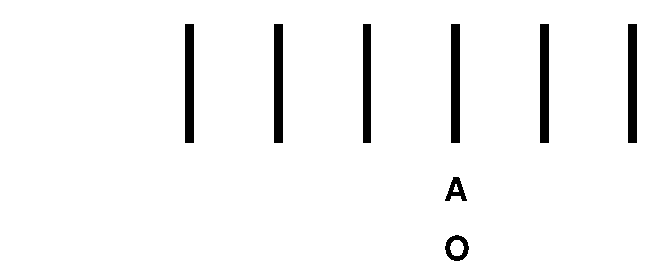
\includegraphics[scale=0.4]{moc}
% \end{SubFloat}%
% \vspace{-10pt}

\begin{SubFloat}{\label{fig:2c}Mapping to physical time}%
% \includegraphics[scale=0.4]{phy.pdf_t}
\scalebox{0.68}{\input{phy.pdf_t}}
\end{SubFloat}%
\caption{Simple SystemJ example and corresponding MoC}
\label{fig:2}
\end{figure}

The perfect synchrony hypothesis is ideal for programming the
synchronous sub-set of SystemJ. Unfortunately, every \textit{micro-step}
requires real-time to compute. Formally, execution of every micro-step
in the logical zero time requires $\delta$ physical time. Time for a
logical tick can thus be summarized as $\Delta = \mathcal{F} (\delta)$,
where $\mathcal{F}$ is some function dependent upon the
\underline{schedule}. We call $\Delta$ the reaction time. Depending upon
the amount of computation required and schedule, $\Delta$ can vary,
hence, in order to satisfy the implicit restriction imposed by the
synchrony hypothesis -- no input event \textit{from the environment} can
be missed -- one needs to calculate the \textit{Worst Case Reaction
  Time} (WCRT) and the resultant WCRT needs to be smaller than the time
between any two consecutive events on any input, else the synchrony
hypothesis is violated. Techniques for calculating the WCRT of
synchronous programs~\cite{boldt07} exist and this analysis is not the
focus of this paper. The opposite of the WCRT is the \textit{Best Case
  Reaction Time} (BCRT), we denote the WCRT and BCRT in
Figure~\ref{fig:2c} using \texttt{W} and \texttt{B},
respectively. Figure~\ref{fig:2c} shows a continuously running physical
clock (analogous to a clock in digital hardware), the numerical
annotations on the rising edge of the clock mark the logical ticks from
Figure~\ref{fig:2c}. The subscripts \texttt{s} and \texttt{e} for the
numbers show the start and end of the logical ticks, respectively. The
end of a logical tick and the start of the next logical tick happen
together. Figure~\ref{fig:2c} shows the mapping of the logical time to
the physical time. For example, the logical tick \texttt{1} starts at
the first rising edge and completes at the second rising edge of the
physical clock, whereas logical tick \texttt{4} starts at the $4^{th}$
rising edge, but finishes at the $6^{th}$ rising edge of the physical
clock. This difference can be accounted for by the Java computations
required when signal \texttt{A} is input by the environment (see
Figure~\ref{fig:2a}). This elasticity is inherent (and elegant) to both
Esterel and SystemJ.

% We now present a lemma with proof sketch (due to lack of space) that we
% require for the rest of the paper and is special to SystemJ, being a
% GALS language.

% \begin{lemma}
%   WCRT and BCRT analysis are invariant to values of conditional
%   expressions.
% \end{lemma}

% \begin{proof}
%   The physical time ($\delta$) taken by a conditional expression is at
%   best affected by the type rather than the value of the
%   conditional. Example, comparing the value of 2 floats might take
%   longer than comparing the value of 2 integer types on some given
%   platform. But, the time taken by the comparison instruction is
%   invariant to the value itself.
% \end{proof}

% \begin{lemma}
%   WCRT and BCRT analysis are invariant to channel communication.
% \end{lemma}
% \begin{proof}
%   LATER ....
% \end{proof}


%%% Local Variables: 
%%% mode: latex
%%% TeX-master: "paper"
%%% End: 

\section{Introducing real-time in SystemJ}
\label{sec:intr-real-time}

We introduce a single \textit{derived} (built from kernel constructs)
statement called \mbox{\texttt{delay (M..N)}} in the SystemJ language
for real-time control. The resolution of the delay statement is of
secondary concern and is dependent upon the execution platform.

\subsection{Semantics of the delay statement}
\label{sec:semant-delay-stat}

Given a SystemJ program: \texttt{delay (M..N); p}, where $M \in
\mathbb{Q}^{>0}$ and $N \in \mathbb{Q}^{>0}$, statement $p$ is executed
after real-time delay of $\tau$ units, such that, $M \leq \tau \leq N$.

We also introduce two variants of the derived statement \texttt{delay}.
\begin{enumerate*}
\item Given a SystemJ program \texttt{delay (M); p}, where $M \in
  \mathbb{Q}^{>0}$, statement $p$ is executed after real-time delay of
  $\tau$ units, such that, $M \leq \tau < \infty$. It is important to
  note that the lower bound of the delay construct $M$ is \textit{not}
  an exact delay, but rather the control is allowed to proceed to the
  next statement anytime after the delay of time $M$.
\item Given a SystemJ program \texttt{delay (M..M); p}, where $M \in
  \mathbb{Q}^{>0}$, statement $p$ is executed after real-time delay of
  $\tau$ units, such that, $M \leq \tau \leq M$. In this variant, the
  delay is exact.
\end{enumerate*}

The aforementioned variants are special cases of the general case
\texttt{delay (M..N)}.

\subsection{Rewriting the \texttt{delay} statement}
\label{sec:rewr-delay-stat}

The introduced \texttt{delay} construct is not a kernel construct, but a
\textit{derived} construct built from the kernel constructs
(Table~\ref{tab:1}) in SystemJ. Figure~\ref{fig:3} gives the rewrite of
the \texttt{delay} construct to kernel statements.

\begin{figure}[tb]
    \begin{minipage}{\textwidth}
      \begin{scriptsize}
\begin{verbatim}
trap(T){
 int x = 0;
 while(true){
  x = x + 1;
  pause;
  if(x == d) exit (T); //wait for "d" ticks
 } // d is the number of logical ticks calculated
} // by Algorithm 1
\end{verbatim}
      \end{scriptsize}
    \end{minipage}
    \caption{The rewrite of \texttt{delay} construct}
    \label{fig:3}
\end{figure}

The fundamental observation is that real-time is converted into logical
time via the \texttt{pause} construct. The rewrite basically maps the
physical notion of time back to the elegant logical notion of time. The
rewrite \textit{delays} a certain number of logical ticks, before
proceeding to the next statement. The number of logical ticks
\texttt{``d''} to \textit{delay} (Figure~\ref{fig:3}) is determined by
the compiler statically at compile time. The value of \texttt{d} is
intricately tied with the WCRT and BCRT of the program and hence the
execution platform.

\subsection{Finding the logical delay \texttt{d}}
\label{sec:find-logic-delay}

\begin{algorithm}[t!]
  \begin{minipage}{1.0\linewidth}
    \SetAlgoLined
    \KwData{WCRT, BCRT, $M \in \mathbb{Q}^{>0}$, $N \in \mathbb{Q}^{>0}$}
    \KwResult{d}
    let $l_1 \leftarrow \lceil \frac{M}{WCRT} \rceil$\;
    let $l_2 \leftarrow \lceil \frac{M}{BCRT} \rceil$\;
    let $u_1 \leftarrow \lfloor \frac{N}{WCRT} \rfloor$\;
    let $u_2 \leftarrow \lfloor \frac{N}{BCRT} \rfloor$\;
    let $F:(l_1,u_1) \rightarrow S_1$\;
    let $F:(l_2,u_2) \rightarrow S_2$\;
    let $D \leftarrow S_1 \cap S_2$\;
    \Return (some $d \in D$)\;
    \caption{Finding the value of \texttt{d}}
    \label{alg:1}
  \end{minipage}
\end{algorithm}

The computation of \texttt{d} is shown in Algorithm~\ref{alg:1}. This
algorithm is carried out for each CD (in SystemJ) or a synchronous
program individually. \textit{The fundamental observation is -- the
  reaction time for each logical tick is elastic -- varying only between
  the BCRT and the WCRT, thus any number of logical ticks \texttt{d}
  that map to the required real-time \texttt{delay} should be chosen in
  such a way that they are invariant to this elasticity.}

Our algorithm takes as input: WCRT, BCRT, and the lower and upper bounds
$M$ and $N$, respectively of the \texttt{delay} construct. We first
divide $M$ and $N$ with the BCRT and WCRT, respectively. This division
gives us the number of individual logical ticks required to delay the CD
(or synchronous program) by the real-time specification. We always
$ceil$ when dividing $M$ and $floor$ when dividing $N$ to make sure that
the resultant values are integers (in domain $\mathbb{N}^{>0}$) and
these functions guarantee that the resultant logical ticks result in
real-time delays between the required range $M-N$. Next, a function $F$
maps these calculated values to a set of equidistant integer points
(values) separated by a unit value -- these points represent all the
logical ticks running at the WCRT and the BCRT, respectively that
satisfy the real-time delay requirements. The intersection of these two
sets gives all the logical ticks that satisfy the real-time requirements
invariant of the logical time and its elasticity.

Let us revisit our motivating example to illustrate the algorithm. From
Figure~\ref{fig:1} we know that $M$ is 50.3 ms and $N$ is 200.3 ms,
respectively. Let the WCRT and BCRT be: 0.112 ms and 0.0334 ms,
respectively. Thus, the algorithm proceeds as follows:

\begin{enumerate*}
\item $l_1 \leftarrow \lceil 50.3/0.112 \rceil$ and $u_1 \leftarrow
  \lfloor 200.3/0.112 \rfloor$. $l_1 = 450$ and $u_1 = 1788$. We first
  calculate the logical ticks that are always running at the WCRT and
  satisfy the required real-time delay.
\item $l_2 \leftarrow \lceil 50.3/0.0334 \rceil$ and $u_2 \leftarrow
  \lfloor 200.3/0.0334 \rfloor$. $l_1 = 1506$ and $u_1 = 5997$. We do
  the same for the BCRT case.
\item $S_1 = [450..1788]$ and $S_2 =[1506,5997]$. We then map the
  resultant bounds to linear points. Sets $S_1$ and $S_2$ represent
  logical ticks that running at the WCRT and BCRT, respectively always
  satisfy the required real-time constraints.
\item $D = S_1 \cap S_2$, $D = [1506,1788]$. Finally, the intersection
  of the two sets gives the set $D$ from which we can choose any value
  for \texttt{d}.
\end{enumerate*}

The resultant value for \texttt{d} gives the number of logical ticks,
which can run at any physical clock-speed, bounded by the BCRT and the
WCRT of the program and still result in the desired real-time delay. We
think this is an elegant solution, because the technique provides
hard-real time guarantees while preserving the essence (elastic logical
tick) of synchronous and GALS programming prescribed by SystemJ and
Esterel style languages. Moreover, this technique considers non
maximal-parallelism, i.e., the delays in logical ticks is calculated
after scheduling of CDs or synchronous programs has been performed. To
our knowledge we are the first to do so.

\subsection{Extending the technique to variants of \texttt{delay}}
\label{sec:extend-tehcn-vari}

\paragraph{The \texttt{delay(M)} construct}
\label{sec:extend-techn-vari}

The \texttt{delay(M)} variant is easily accommodated in the
technique. All one needs to do is find the set $S_1$ and choose a value
from this set.

\paragraph{The \texttt{delay(M..M)} construct}
\label{sec:extend-techn-vari}

The \texttt{delay(M..M)} variant is a little more interesting. Like
before we find sets $S_1$ and $S_2$, and find the intersection of the
two sets to get the value of \texttt{d}. It is possible (and often
likely, as suggested by our experiments in
Section~\ref{sec:experimental-results}) that the resultant set $D$ is
empty (also possible in the case of \texttt{delay(M..N)}, but never
possible in case of \texttt{delay(M)}). In such a case, we automatically
\textit{relax} the upper bound of the \texttt{delay} statement.

\paragraph{Relaxation of the upper real-time bound}
\label{sec:over-appr-relax}

The relaxation technique is shown in Algorithm~\ref{alg:2}.
  
\begin{algorithm}[t!]
  \begin{minipage}{1.0\linewidth}
    \SetAlgoLined
    \KwData{$S_2$, $D$, WCRT}
    \KwResult{d}
    \If {$D = \emptyset$} {
      let $j_{0}$ be the first element of set $S_2$, s.t., $|S_2|=Q$\;
      \ShowLn let $N \leftarrow WCRT \times j_0$\;
      let $d \leftarrow j_0$\;
    }
    \Return d\;
    \caption{Calculating the minimum relaxation of the upper real-time
      bound}
    \label{alg:2}
  \end{minipage}
\end{algorithm}


This algorithm results in the smallest relaxation required for the
real-time delay to be satisfied. The algorithm takes as input the WCRT
and set $S_2$, recall that set $S_2$ represents the logical ticks
required to satisfy the real-time requirement at the BCRT. We take the
very first value from set $S_2$ and multiply it with the WCRT to get the
relaxation $N$. The first element of set $S_2$ is returned as the
logical tick delay \texttt{d}.

The fundamental observation is that we have to delay for a minimum of
$M$ units of real-time, hence, under-approximation is out of
question. We can still over-approximate, but to reduce the resultant
error, we should over-approximate by least possible value, which is the
lower bound of set $S_2$. Thus, the lower bound is considered to be the
only element shared between the two sets $S_1$ and $S_2$ and
accordingly, the upper real-time bound is relaxed by the multiplication
of WCRT and the first element of set $S_2$.


\subsection{Programming using the delay construct}
\label{sec:progr-using-delay}

In this section we provide a number of examples to show the different
types of real-time programming paradigms that can be incorporated into
the GALS (and its sub-set synchronous) programming model.

\subsubsection{Non-deterministic time}
\label{sec:non-determ-time}

Many real-world systems require non-deterministic timing
constructs. Where the exact real-time delay is not known or should not
be known apriori. One such system is our motivating example -- the human
response time system.

% Another is a printer-spooler example borrowed from timed
% CSP~\cite{Schneider:1999:CRT:555233}. The spooler and printer need to
% synchronize using channels. The printer might be unable to print
% depending upon the paper tray, similarly, spooler might take sometime
% to send the job depending upon its size. Such real-time constraints
% can be modeled in SystemJ as below:

% \begin{scriptsize}
  
% \begin{verbatim}
% {await (job); delay (2..10 ms);  //SPOOLER CD
%  send mid(job) delay (1ms);}
% ><
% {receive mid; delay(1..30 ms); //PRINTER CD
%  emit print(#mid);}
% \end{verbatim}
% \end{scriptsize}

\subsubsection{Timeout}
\label{sec:timeout}

There are many instances when one would like to wait on an input from
environment for only a specified amount of time. This can be programmed
as:
% \begin{scriptsize}
\begin{verbatim}
// timeout after 1ms.
trap(T){{await(A);}||{delay(1..1 ms);exit(T);}}
\end{verbatim}
% \end{scriptsize}

\subsubsection{Periodic reactions}
\label{sec:periodic-reactions}

A reaction, or a whole CD, can be programmed to run periodically like
so:

% \begin{scriptsize}
\begin{verbatim}
while(true) { delay ((1..1)ms); emit S; 
 //do something }
\end{verbatim}
% \end{scriptsize}
A periodic reaction (or CD) requires special consideration. Since the
delay statement is converted into \texttt{pause} constructs. One should
not introduce extra \texttt{pause} constructs when building periodic
reactions (or CDs). This is essential since introducing additional
pauses would introduce more logical ticks.

\subsubsection{Interaction of preemption and delays}
\label{sec:inter-preempt-delays}

Preemption plays an important role in reactive languages. One needs to
carefully consider the interplay of \texttt{delay} semantics with the
preemption semantics of reactive languages. Previous attempts at
incorporating delays (using external timers) have only been partially
successful, because of the complex interplay between real-time and
preemption. Consider the simple example below, which models real-time
using external timers as in~\cite{rsh94}.

% \begin{scriptsize}
\begin{verbatim}
suspend{S} {emit START_TIMER(10); await (TIMER); 
 emit O1;}
\end{verbatim}
% \end{scriptsize}

As identified in~\cite{Bourke2009a} the \texttt{suspend} does not play
well with the external timer. The above program sends a signal to an
external timer and waits for 10 ms to pass by. Consider what happens
when signals \texttt{S} and \texttt{TIMER} occur in the same logical
tick, the \texttt{await} statement is never executed (due to suspend)
and hence, we enter a deadlock. Such problems are completely avoided in
our technique, because we convert the real-time delays into logical
delays (\texttt{pause} constructs), which interact well with preemption.

\subsubsection{Interaction of channel communication and delays}
\label{sec:inter-chann-comm}

Channels, used for communication between reactions in asynchronously
running CDs, are an addition in the SystemJ language. Like interaction
of preemption and delays, conversion of real-time delays to logical
ticks also interacts well with channel rendezvous, because the semantics
of interaction are well defined~\cite{amal10}. More importantly, we need
to consider the interplay of channel communication and WCRT/BCRT
analysis. Since, channel communication does not stop logical time
(see~\cite{amal10}) WCRT/BCRT are unaffected by channel
communication. % The response time to input signals \textit{is} though!
% But, we are unconcerned with the response time, analysis in this paper
% and it remains a future research avenue.

%%% Local Variables: 
%%% mode: latex
%%% TeX-master: "paper"
%%% End: 



\section{Experimental results}
\label{sec:experimental-results}

\begin{center}
\scalebox{0.9}{
\begin{tabular}{|c| c | c | c | c | c | c | c |}
	\cline{4-8}
	\multicolumn{3}{c|}{}											& HRTCS 		& Motor 		  & Robot 			  & AECS/CD1  		   & AECS/CD2\\ \hline
	\multirow{12}{*}{JOP} 		& \multicolumn{2}{|c|}{BCRT} 		&0.0334 ms 		& 0.0361 ms		  & 0.0325 ms		  & 0.1683 ms		   & 0.1881 ms\\ \cline{2-8}   
								& \multicolumn{2}{|c|}{WCRT} 		&0.1120 ms 		& 0.1116 ms		  & 0.0601 ms		  & 0.7147 ms		   & 1.0115 ms\\ \cline{2-8} 
								& \multirow{2}{*}{Delay 1}	 & M..N &50.3-200.3 ms 	& 2.4-7.4772 ms	  & 1230-2274.0263 ms & 10000-42473.2197 ms& 10000-53772.0045 ms \\ \cline{3-8} 
								&			   & d			 		&1506-1787  	& 67 			  & 37861			  & 59427		       &53160\\ \cline{2-8}
								& \multirow{2}{*}{Delay 2}	 & M..N & 	N/A 		& 1.667-5.2452 ms & N/A				  & N/A 			   &10000-53772.0045 ms\\ \cline{3-8} 
								&			   & d			 		& 	N/A	 		& 47			  & N/A				  & N/A       		   &53160\\ \cline{2-8}
								& \multirow{2}{*}{Delay 3}	 & M..N & 	N/A	 		& 0.05-0.2232 ms  & N/A				  & N/A       		   &N/A\\ \cline{3-8} 
								&			   & d			 		& 	N/A	 		& 2		      	  &	N/A				  & N/A       		   &N/A\\ \cline{2-8}
								& \multirow{2}{*}{Delay 4}	 & M..N & 	N/A	 		& 0.3-1.0044 ms   & N/A				  &	N/A       		   &N/A\\ \cline{3-8} 
								&			   & d				 	& 	N/A	 		& 9				  & N/A				  &	N/A      		   &N/A\\ \cline{2-8}
								& \multirow{2}{*}{Delay 5}	 & M..N & 	N/A	 		& 0.733-2.3436 ms & N/A				  &	N/A      		   &N/A\\ \cline{3-8} 
								&			   & d			 		& 	N/A	 		& 21 			  &	N/A				  & N/A      		   &N/A\\ \hline
	\multirow{12}{*}{TP-JOP} 	& \multicolumn{2}{|c|}{BCRT} 		&0.0028 ms 		& 0.0060 ms		  & 0.0011 ms		  & 0.0532 ms		   & 0.0292 ms\\ \cline{2-8}   
								& \multicolumn{2}{|c|}{WCRT} 		&0.0329 ms 		& 0.0393 ms		  & 0.0361 ms		  & 0.5072 ms		   & 0.8388 ms\\ \cline{2-8} 
								& \multirow{2}{*}{Delay 1}	 & M..N &50.3-600.3 ms 	& 2.4-15.6265 ms  & 1230-42317.8276 ms& 10000-95358.8578 ms& 10000-287757.9834 ms \\ \cline{3-8} 
								&			   & d			 		&18209-18232 	& 398 			  & 1171429			  & 188015		       &343054\\ \cline{2-8}
								& \multirow{2}{*}{Delay 2}	 & M..N & 	N/A 		& 1.667-10.8757 ms& N/A				  & N/A 			   &10000-287757.9834 ms\\ \cline{3-8} 
								&			   & d			 		& 	N/A	 		& 277			  & N/A				  & N/A       		   &343054\\ \cline{2-8}
								& \multirow{2}{*}{Delay 3}	 & M..N & 	N/A	 		& 0.05-0.3534 ms  & N/A				  & N/A       		   &N/A\\ \cline{3-8} 
								&			   & d			 		& 	N/A	 		& 9		      	  &	N/A				  & N/A       		   &N/A\\ \cline{2-8}
								& \multirow{2}{*}{Delay 4}	 & M..N & 	N/A	 		& 0.3-1.9631 ms   & N/A				  &	N/A       		   &N/A\\ \cline{3-8} 
								&			   & d				 	& 	N/A	 		& 50			  & N/A				  &	N/A      		   &N/A\\ \cline{2-8}
								& \multirow{2}{*}{Delay 5}	 & M..N & 	N/A	 		& 0.733-4.79 ms   & N/A				  &	N/A      		   &N/A\\ \cline{3-8} 
								&			   & d			 		& 	N/A	 		& 122 			  &	N/A				  & N/A      		   &N/A\\ \cline{2-8}
	\hline
\end{tabular}
}
\end{center}


aa

%%% Local Variables: 
%%% mode: latex
%%% TeX-master: "paper"
%%% End: 



\section{Related work}
\label{sec:related-work}


A number of studies have been performed when it comes to integrating
real-time directly as a programming construct in GALS (and its subset
synchronous) reactive languages. The most prominent works in this area
are by Shyamsundar~\cite{rsh94} and Bourke et
al.~\cite{Bourke2009a}. Shyamsundar incorporates real-time using
external timers in \textit{Communicating Reactive Processes} (CRP),
which like SystemJ is an extension of synchronous language Esterel to
asynchorny. But, as mentioned in Section~\ref{sec:inter-preempt-delays},
external timers do not interact well with preemption constructs in these
languages. Bourke et al. introduce real-time as first class constructs
in the Esterel language. They like us provide real-time \texttt{delay}
as first class Esterel programming constructs, and translate them into
Esterel kernel constructs. But, unlike us they do not translate delays
into \texttt{pause} constructs directly. Instead, logical ticks are
generated by using abstract notion of \texttt{event} and \texttt{sample}
platform dependent timers. This notion makes it a complex and inflexible
solution since the number of platform timers with certain resolutions
need to be determined and present on the system for the solution to be
realizable. Moreover, non-deterministic real-time delays and integration
with non-maximal parallelism is not studied at all. Our solution does
not require external timers (like~\cite{rsh94}) or logical notion of
timers (like~\cite{Bourke2009a}). In our solution we calculate the delay
in logical ticks \textit{after} allocation and scheduling, it gives the
compiler developers the chance to optimize for many different criteria
such as computation time, energy, power, etc, without worrying about or
violating the real-time delay specification.

Other works such as Quartz~\cite{glog02} and Bertin et
al.~\cite{Bertin:2000:TVR:1947412.1947439}, also incorporate delay
statements in Esterel using \texttt{pause} and special \textit{pragmas}
(annotations), respectively.  The Quartz solution is targeted at
studying timing properties using model checkers rather than
implementation, like us. The solution introduced by Bertin et
al.~\cite{Bertin:2000:TVR:1947412.1947439} translates real-time pragmas
into Timed automata~\cite{alur94} for model-checking real-time
deadlines. Our solution on the other hand removes all continuous time
elements and produces single discrete time model thereby making the
solution amenable to existing functional and real-time verification
tools developed for reactive languages and more in the spirit of logical
time. Finally, a major difference between Bertin et al. and our approach
is that their approach requires programmers to annotate the time taken
by `C' code fragments manually, this is extremely error prone, we use
static low-level program analysis to find out such times automatically.


%%% Local Variables: 
%%% mode: latex
%%% TeX-master: "paper"
%%% End: 



\section{Conclusion}
\label{sec:concl-future-work}

In this paper we have described a novel way to introduce real-time in
\textit{Globally Asynchronous Locally Synchronous} (GALS) languages, in
particular SystemJ, and their subset the synchronous languages like
Esterel. The fundamental idea is to convert real-time delay into logical
delays (\texttt{pause} construct) that interact well with rest of the
constructs in these languages, especially, preemption and channel
communication. We do \textit{not} need or use external timers to
introduce these real-time delays, instead we depend upon an underlying
platform that is timing analyzable, thereby resolving the problems of
interaction between external timers and preemption. Moreover, we also do
not require specific timer resolutions, thereby making our solution
elegant (in the spirit of GALS/synchronous programming) and flexible. We
rewrite the delay construct into reactive kernel constructs, calculate
the \textit{Worst} and \textit{Best} case reaction times and then
determine \textit{delay} \texttt{d}, number of logical ticks, which is
invariant to the \textit{elasticity} of logical time. To our knowledge
we are the first to introduce precise and imprecise delays in such
languages and show their usefulness in designing real-world systems.


%%% Local Variables: 
%%% mode: latex
%%% TeX-master: "paper"
%%% End: 


\bibliographystyle{plain}
\bibliography{main.bib}
\end{document}
